\chapter{Introduction}
\label{ch:intro}

In this chapter, We will focus on the main subjects of static program analysis. 
Section \ref{sec:comp} we talk about us, the compiler guys. 
Section \ref{sec:analysis} is about the comparison between static and dynamic analysis. 
In the next section \ref{}, we want to show some applications in real life.  

\section{The Compiler Guys and Where We're Going}
\label{sec:comp}

Someone in one place and one time was thinking about how to save time for millions of programmers, and the answer was simple: Let's build a Compiler! The goal of a compiler writer is to bridge the gap between programming languages and the hardware; hence, making programmers more productive. This book is not about creating our own compiler. But, your knowledge of compiler will be welcome here. Well, let's start to present the main goals of this book.

\begin{itemize}
    \item Explain to the student how to transform a program automatically, while preserving its semantics, in such a way the new program is more efficient according to a well-defined metric.
    \item Introduce students to techniques that let them understand a program to a level that would be hardly possible without the help of a machine.
\end{itemize}

Before we start the book. Let's understand the basic of Compiler. Figure \ref{fig:compiler} illustrates where we stay in this book. A Compiler has three main parts:

\begin{itemize}
    \item The front-end is where parsing takes place.
    \item The middle-end is where optimizations and analyses take place.
    \item The back-end is where actual machine code is generated.
\end{itemize}

Static program analysis work, but not limited, in middle-end place. In this book we are going working with LLVM to show the theory works in practice. For example, in this chapter (see the Section \ref{subsec:intro_llvm}) we will see about what LLVM means and how to install the tool in your computer (the simple and the dragon way).  

\begin{figure}[ht]
    \centering
    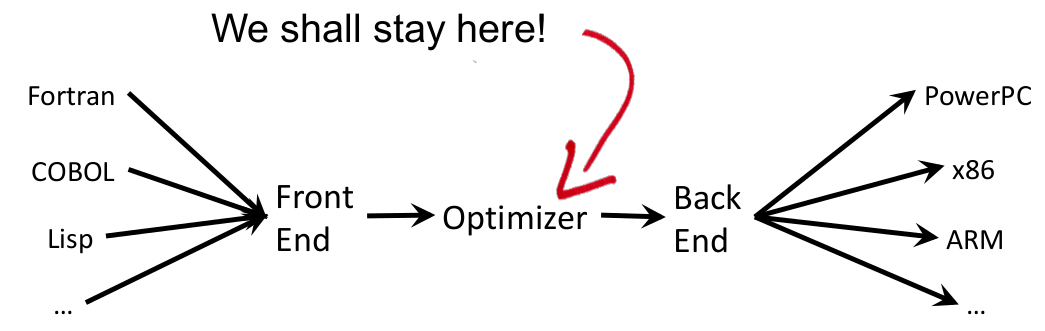
\includegraphics[width=\textwidth]{images/compiler.png}
    \caption{Basic structure of the compiler.}
    \label{fig:compiler}
\end{figure}

\section{Static vs Dynamic Analysis}
\label{sec:analysis}

Static analysis and dynamic analysis are two different approaches used in software testing and analysis. Next, we will discuss the pros and cons of each other.

\textbf{Static analysis} involves examining the source code, design documents, or other artifacts of a software system without executing the code. It focuses on finding defects, vulnerabilities, or potential issues by analyzing the code structure, syntax, and semantics. This analysis is typically performed using specialized tools that can automatically analyze the codebase.

Advantages of Static Analysis:

\begin{itemize}
    \item \textbf{Early bug detection:} Static analysis can identify potential issues in the codebase before the software is even executed, allowing for early bug detection and prevention.
    \item \textbf{Scalability:} It can be applied to large codebases and complex systems, making it suitable for projects of various sizes.
    \item \textbf{Automation:} Static analysis tools can automatically analyze the code, making it efficient for finding common coding mistakes and security vulnerabilities.
    \item \textbf{Code quality improvement:} Static analysis can enforce coding standards and best practices, leading to improved code quality and maintainability.
\end{itemize}

Limitations of Static Analysis:

\begin{itemize}
    \item \textbf{Limited runtime information:} Static analysis cannot capture the complete runtime behavior of the software, making it challenging to detect certain types of issues that only manifest during execution.
    \item \textbf{False positives and negatives:} Static analysis tools may produce false positives (flagging code as problematic when it's not) or false negatives (missing actual issues in the code), requiring manual review and validation.
\end{itemize}

\textbf{Dynamic analysis} involves executing the software and observing its behavior in various scenarios. It aims to uncover defects, performance bottlenecks, memory leaks, and other runtime issues. Dynamic analysis typically requires running the software with specific inputs or test cases to exercise different paths and behaviors.

Advantages of Dynamic Analysis:

\begin{itemize}
    \item \textbf{Real-world simulation:} Dynamic analysis provides insights into how the software behaves in real-world scenarios, helping identify issues that might not be apparent through static analysis alone.
    \item \textbf{Coverage of runtime behaviors:} It captures actual runtime behavior, allowing for the detection of issues related to timing, concurrency, memory management, and interactions with external systems.
    \item \textbf{Profiling and performance analysis:} Dynamic analysis tools can measure performance metrics, such as execution time and memory usage, and help identify performance bottlenecks.
\end{itemize}

Limitations of Dynamic Analysis:

\begin{itemize}
    \item \textbf{Late bug detection:} Dynamic analysis detects issues during or after execution, which means that bugs may go undetected until the software is executed.
    \item \textbf{Incomplete coverage:} It may be challenging to exercise all possible execution paths, making it difficult to achieve complete coverage of the software.
    \item \textbf{Time-consuming:} Dynamic analysis requires executing the software, which can be time-consuming, especially for large systems or complex test scenarios.
\end{itemize}

In practice, both static and dynamic analysis techniques complement each other and are often used in combination to achieve comprehensive software testing and analysis. Static analysis helps catch potential issues early in the development process, while dynamic analysis provides insights into the actual runtime behavior and helps uncover issues that may only manifest during execution. 

In this book, we will focus on techniques for static analysis, but there will be a release in the future, a book where It focuses on dynamic analysis. 

\subsection{Program Optimization}

Program optimization refers to the process of improving the performance, efficiency, or other desired characteristics of a software program. Optimization techniques aim to reduce the program's resource usage, such as CPU time, memory consumption, or network bandwidth, while still achieving the desired functionality. Here's an example to illustrate program optimization:

Let's consider a simple example of a function that calculates the sum of numbers in an array using a basic iterative approach:

\begin{lstlisting}[language=Python]
def sum_array(arr):
    result = 0
    for num in arr:
        result += num
    return result
\end{lstlisting}

While this code works correctly, it may not be optimal in terms of performance. If the array has a large number of elements, the iterative approach can be inefficient. We can optimize this code by using a more efficient algorithm, such as a divide-and-conquer approach. Here's an optimized version using recursion:

\begin{lstlisting}[language=Python]
def sum_array_optimized(arr):
    if len(arr) == 1:
        return arr[0]
    else:
        mid = len(arr) // 2
        left_sum = sum_array_optimized(arr[:mid])
        right_sum = sum_array_optimized(arr[mid:])
        return left_sum + right_sum
\end{lstlisting}

In this optimized code, we divide the array into smaller halves recursively until we reach arrays of size 1. Then, we sum the elements of each small array and return the final result. This approach reduces the number of operations required and can be more efficient for large arrays.

It's important to note that program optimization may involve trade-offs. While optimization can improve certain aspects of the program, it may also make the code more complex or harder to understand. This is one of the goals of the techniques that we will see in this book is to optimize programs without the programmer interfering in the code. 

There are many ways to optimize programs. We will see some of these techniques:

\begin{itemize}
    \item Copy elimination
    \item Constant propagation
    \item Lazy Code Motion
    \item Register Allocation
    \item Loop Unrolling
    \item Value Numbering
    \item Strength Reduction
    \item and others more
\end{itemize}

\subsection{Bug Finding}
\label{subsec:bug}

Bug finding refers to the process of identifying and fixing bugs, defects, or errors in software applications. Bugs can cause the software to behave unexpectedly, produce incorrect results, or crash. Bug finding techniques are used to locate and diagnose these issues, allowing developers to resolve them and improve the overall quality and reliability of the software. 

Static analysis tools analyzes the source code or other artifacts without executing the software. They perform automated checks for coding errors, potential bugs, or violations of coding standards. These tools can identify issues such as uninitialized variables, dead code, buffer overflows, or potential security vulnerabilities. Static analysis can be an effective way to catch bugs early in the development process. By the other hand, Dynamic analysis techniques involve running the software with specific inputs or test cases to observe its behavior during execution. These techniques include techniques like runtime monitoring, profiling, and memory analysis. Dynamic analysis can uncover bugs related to performance bottlenecks, memory leaks, concurrency issues, or unexpected behavior during runtime.

Therefore, Compiler analyses are very useful to fine, and sometimes fix, bugs in programs. For example, The snippet code in C++ below there is a security bug. Could you spot a security bug in this program? Don't worry if you could not, the answer it'll be shown during the book.

\begin{lstlisting}[language=C++]
void read_matrix(int* data, char w, char h) {
    char burf_size = w * h;
    if (buf_size < BUF_SIZE) {
        int c0, c1;
        int buf[BUF_SIZE];
        for (c0 = 0; c0 < h; c0++) {
            for (c1 = 0; c1 < w; c1++) {
                int index = c0 * w + c1;
                buf[index] = data[index];
            }
        }
        process(buf);
    }
}
\end{lstlisting}

The main topics when you study static program analyses about the bug finding, but not limited, are:

\begin{itemize}
    \item Null pointer deference
    \item Array out-of-bounds access
    \item Invalid Class Cast
    \item Tainted Flow Vulnerabilities
    \item Integer Overflows
    \item Information leaks
\end{itemize}

\subsection{Introduction to LLVM}
\label{subsec:intro_llvm}

LLVM (Low-Level Virtual Machine) is an open-source compiler infrastructure project that provides a collection of modular compiler and toolchain technologies. Originally developed at the University of Illinois at Urbana-Champaign by Chris Lattner, LLVM has grown into a widely adopted framework for building compilers, code optimization tools, and runtime environments. 

The Key Components of LLVM are:

\begin{itemize}
    \item \textbf{LLVM Core:} The core component of LLVM is a collection of libraries and APIs that provide the foundation for building compilers and other tools. It includes components for front-end parsing, intermediate representation (IR) generation, optimization, and code generation.
    \item \textbf{Clang:} Clang is a front-end C, C++, and Objective-C compiler built using LLVM. It aims to provide high-quality diagnostics, fast compilation, and compatibility with various C/C++ standards. Clang leverages LLVM's modular architecture and infrastructure, making it a popular choice for many developers.
    \item \textbf{LLVM IR:} LLVM uses an intermediate representation (IR) called LLVM IR. It is a platform-independent, typed, and low-level representation of code that sits between the source code and the machine code. LLVM IR allows for various optimizations to be performed on the code before generating the final machine code.
    \item \textbf{Optimization Framework:} LLVM provides a powerful optimization framework that performs a wide range of program transformations to improve code quality and performance. It includes optimizations such as constant propagation, loop optimizations, inlining, dead code elimination, and many others.
    \item \textbf{Just-in-Time Compilation (JIT):} LLVM supports Just-in-Time Compilation, allowing dynamic compilation and execution of code at runtime. This is particularly useful in dynamic languages and environments where code needs to be compiled and optimized on the fly.
    \item \textbf{Target Backends:} LLVM supports multiple target architectures and provides backends for generating machine code for different hardware platforms. This allows LLVM to be used for compiling code for various processors, including x86, ARM, MIPS, PowerPC, and more.
    \item \textbf{Toolchain Integration:} LLVM integrates with various development tools and platforms, making it possible to use LLVM as part of a complete toolchain. It can be integrated with build systems, debuggers, profilers, and other development tools.
\end{itemize}

LLVM is widely used in both academia and industry for various purposes, including compiler research, language implementation, code optimization, and tool development. Its modular and flexible architecture, along with its extensive optimization capabilities, make it a popular choice for building high-performance compilers and software tools. Let's see how to install in your machine in the next section.

\subsection{Installing LLVM}

We suppose that you use an OS based on the Linux kernel. You can use WSL from Windows as well. For user's Apple, the process is pretty similar on Linux.
Your first step is to clone the LLVM from GitHub with the command below:

\begin{verbatim}
    $ git clone https://github.com/llvm/llvm-project
\end{verbatim}

Next step, It'll created inside the llvm-project directory, the build folder. 

\begin{verbatim}
    $ mkdir -p build
\end{verbatim}

After that, we will compile using the CMakefile builder. The command below will build using this build:

\begin{verbatim}
    $ cmake -DLLVM_ENABLE_PROJECTS="clang;clang-tools;
    compiler-rt" -DCMAKE_BUILD_TYPE=Debug -G "Unix Makefiles" ../llvm
\end{verbatim}

Or you can use the Ninja builder:

\begin{verbatim}
    $ cmake -DLLVM_ENABLE_PROJECTS="clang;clang-tools;
    compiler-rt" -DCMAKE_BUILD_TYPE=Debug -G "Ninja" ../llvm
\end{verbatim}

This process takes a long time. With a good machine, several cores, and a lot of RAM memory, this process can take approximately 20–30 minutes. After this process, congratulation on your machine you have installed LLVM, and you're ready for the next chapter. 

Any doubts about the process, you can read the getting started from \hyperlink{https://llvm.org/docs/GettingStarted.html}{LLVM page}.